\documentclass{standalone}
\usepackage{tikz}
\usepackage{pgfplots}
\pgfplotsset{width=32cm,height=18cm,compat=1.3}
\pgfplotsset{every tick label/.append style={font=\Huge}}
\usepackage{filecontents}

\usetikzlibrary{patterns}

\definecolor{citrine}{rgb}{0.89, 0.82, 0.04}

\begin{document}
	\centering
		\vspace{1.5em}
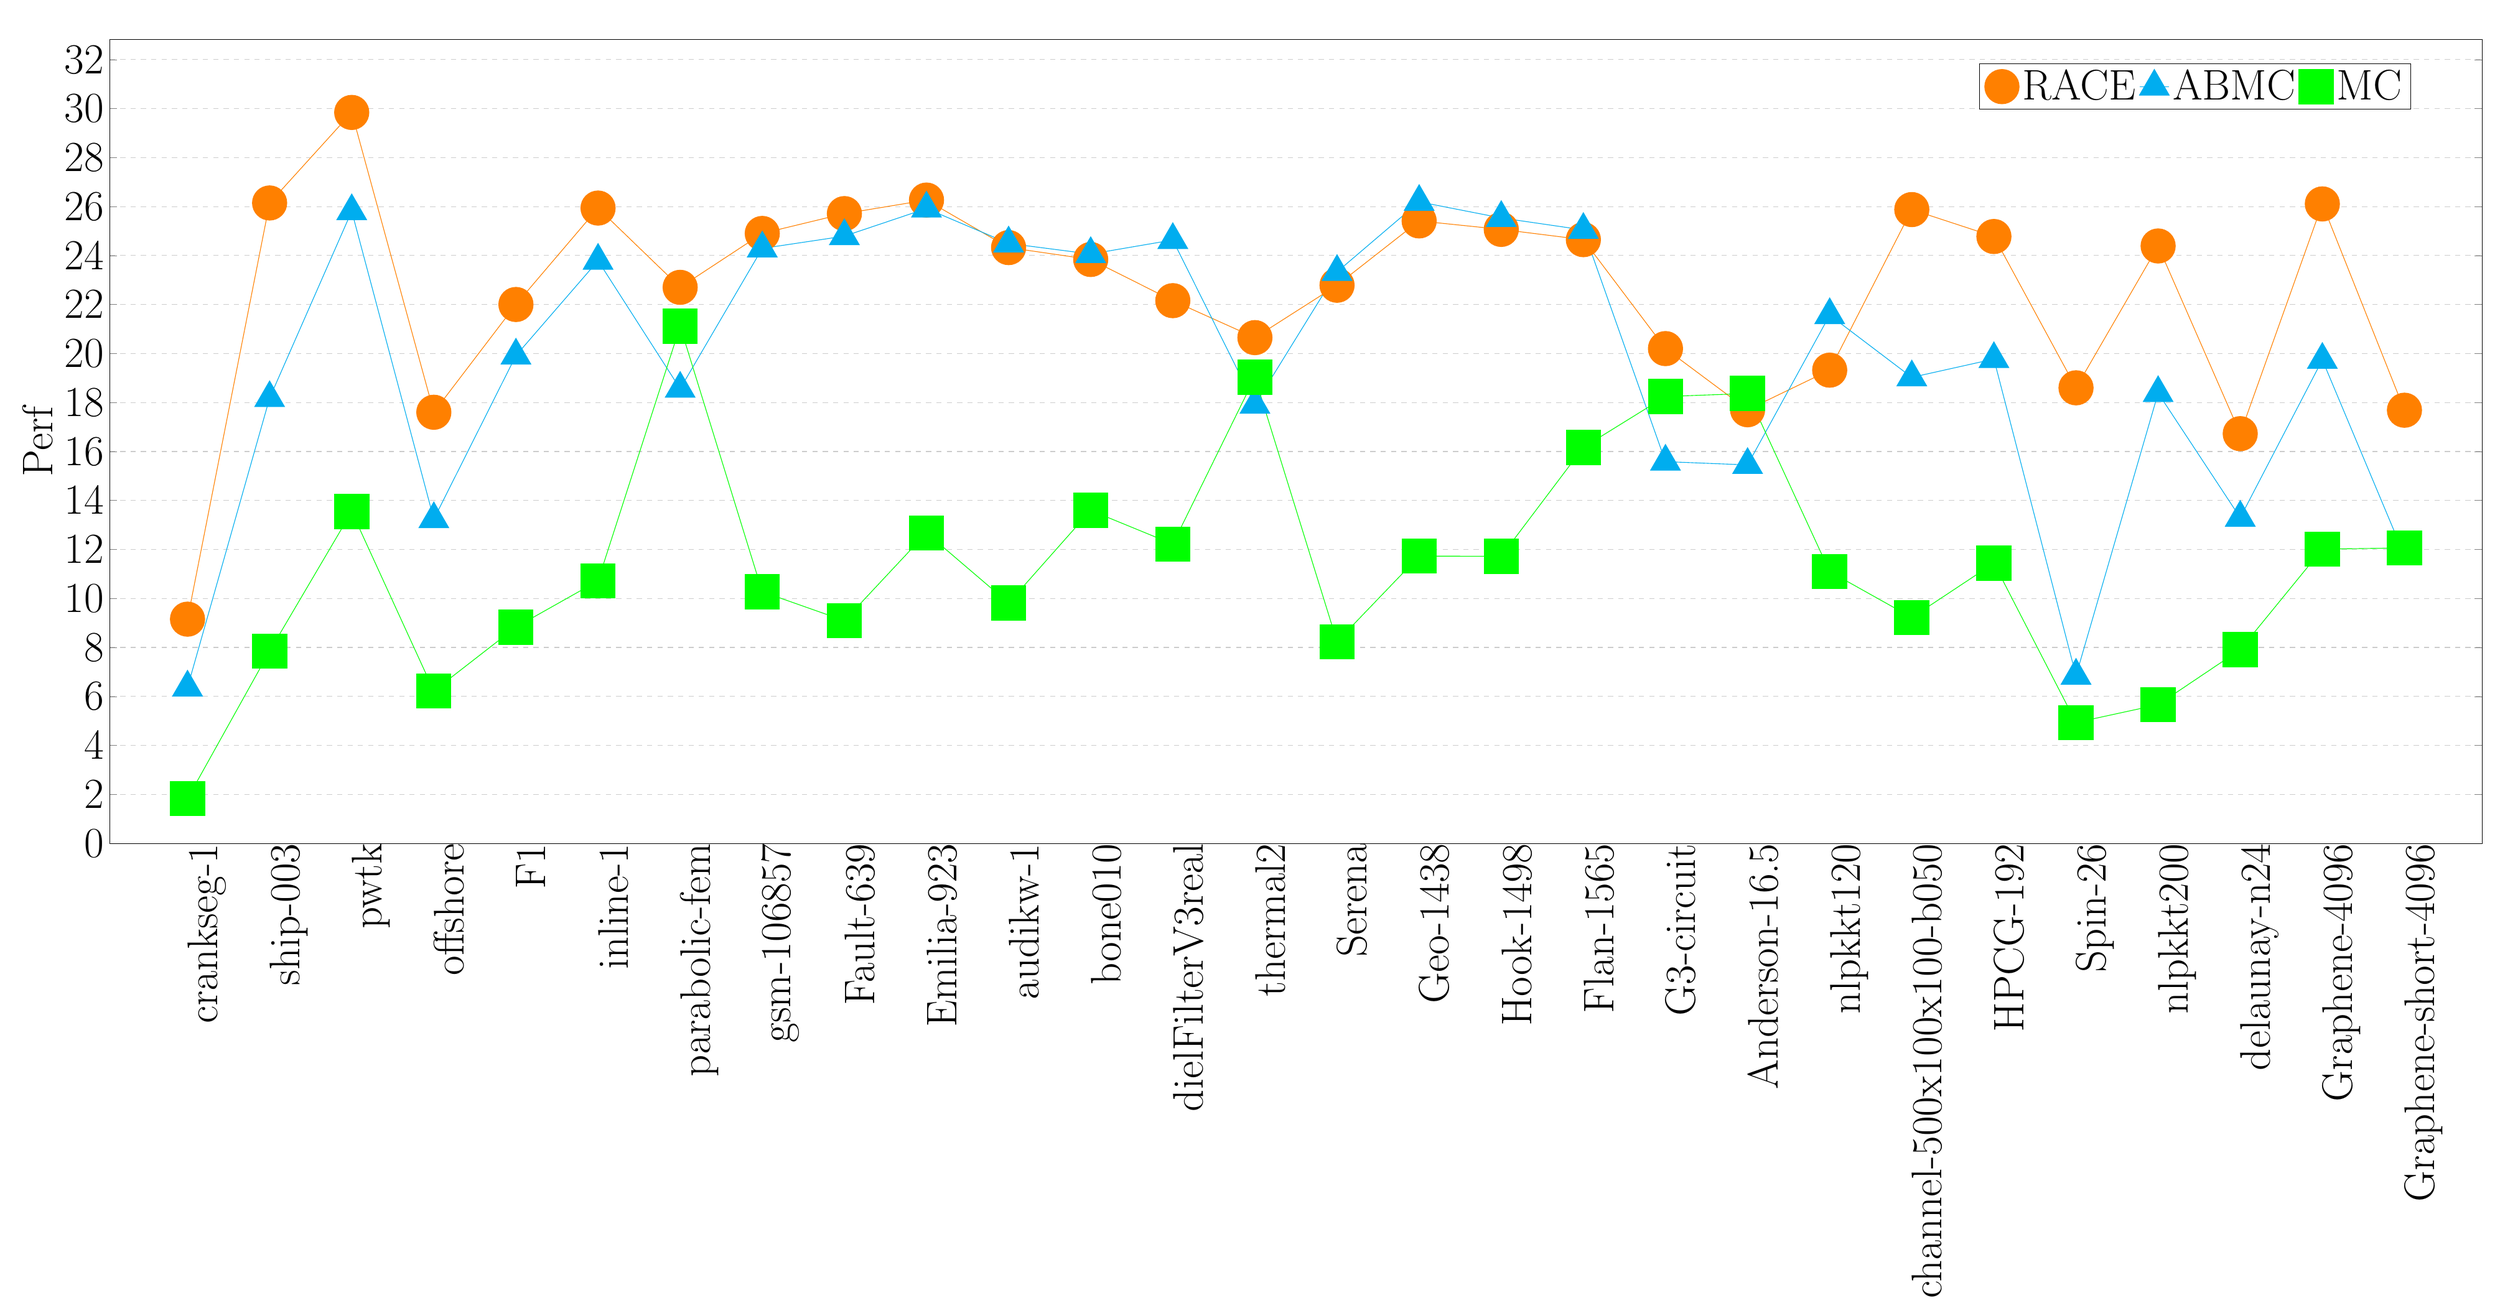
\begin{tikzpicture}
		%	\node at (13.25,15) {\LARGE{}};
			\begin{axis}[
		%	xmin=0.25, xmax=7.25,
			ymin=0, %ymax=3.25,
			xtick={1, 2, 3, 4, 5, 6, 7, 8, 9, 10, 11, 12, 13, 14, 15, 16, 17, 18, 19, 20, 21, 22, 23, 24, 25, 26, 27, 28},
		%	ytick={0,0.5,1,1.5,2,2.5,3},
			xticklabels={crankseg-1, ship-003, pwtk, offshore, F1, inline-1, parabolic-fem, gsm-106857, Fault-639, Emilia-923, audikw-1, bone010, dielFilterV3real, thermal2, Serena, Geo-1438, Hook-1498, Flan-1565, G3-circuit, Anderson-16.5, nlpkkt120, channel-500x100x100-b050, HPCG-192, Spin-26, nlpkkt200, delaunay-n24, Graphene-4096, Graphene-short-4096},
			width  = 50cm,
			height = 18cm,
			major x tick style = transparent,
			%	minor ytick={1, 5, 10, 15, 20, 25, 30 ,35,40},
			grid = minor,	
			%add_bar_commands
			ymajorgrids = true,
			grid style={dashed, gray!40},
			ylabel = {\Huge{Perf}},
		%	symbolic x coords={Graphene-2048-2048, Graphene-4096-4096, Spin-24-24-24},
			x tick label style={rotate=90, anchor=north east, inner sep=0mm, font={\Huge}},
			tick label style={font={\Huge}},
			scaled y ticks = false,
			enlarge x limits=0.035,
			legend cell align=left,
			legend style={font=\Huge},
			legend columns=-1,
			legend style={
				%at={(1,1.05)},
				%anchor=south east,
				%column sep=1ex,
				legend pos=north east
			},
			%spl_legend_code
			title= {\Huge\scalebox{1.5}{{}}}
			]

\addplot[ mark=*, mark size=10pt, mark options={orange}, draw=orange ] plot coordinates{(1,9.154600) (2,26.146805) (3,29.843171) (4,17.602417) (5,22.002052) (6,25.939085) (7,22.701878) (8,24.902989) (9,25.712719) (10,26.265544) (11,24.325379) (12,23.839610) (13,22.158249) (14,20.649656) (15,22.787833) (16,25.413874) (17,25.068277) (18,24.649242) (19,20.201273) (20,17.704550) (21,19.321052) (22,25.877076) (23,24.777495) (24,18.599889) (25,24.390948) (26,16.727340) (27,26.108377) (28,17.685267)};
\addplot[ mark=triangle*, mark size=10pt, mark options={cyan}, draw=cyan ] plot coordinates{(1,6.365507) (2,18.180514) (3,25.812192) (4,13.238024) (5,19.917146) (6,23.789440) (7,18.562404) (8,24.291373) (9,24.792787) (10,25.920335) (11,24.495287) (12,24.061832) (13,24.635656) (14,17.907685) (15,23.332912) (16,26.192504) (17,25.536124) (18,25.047345) (19,15.585629) (20,15.451611) (21,21.567721) (22,19.027449) (23,19.774422) (24,6.846313) (25,18.385375) (26,13.296630) (27,19.742625) (28,11.755171)};
\addplot[ mark=square*, mark size=10pt, mark options={green}, draw=green ] plot coordinates{(1,1.829046) (2,7.847925) (3,13.545971) (4,6.225119) (5,8.831318) (6,10.718812) (7,21.114680) (8,10.274120) (9,9.092548) (10,12.677173) (11,9.812284) (12,13.595008) (13,12.218950) (14,19.037512) (15,8.235745) (16,11.727714) (17,11.722994) (18,16.168485) (19,18.244402) (20,18.367932) (21,11.097530) (22,9.221154) (23,11.439729) (24,4.933386) (25,5.661606) (26,7.910617) (27,12.016716) (28,12.061076)};
	%addplot cmd

	\legend{RACE, ABMC, MC}

	\end{axis}			
\end{tikzpicture}

\end{document}

